\documentclass{beamer}
\usepackage{beamerthemeshadow}
\usepackage{graphicx}
\usepackage[english,serbian]{babel}
\usepackage{color}
\usepackage[utf8]{inputenc}
\usepackage{hyperref}
\definecolor{darkblue}{rgb}{0.11,0.27,0.55}
\setbeamercolor{structure}{fg=darkblue}

\def\d{{\fontencoding{T1}\selectfont\dj}}
\def\D{{\fontencoding{T1}\selectfont\DJ}}

\title{Vrste beskonačnosti. Paradoks Hilbertovog hotela}
\subtitle{-- Tehničko i naučno pisanje --}
\author{Milica Zubljić, Dimitrije Spasojević, Branko Katanić, Luka Tonić}
\institute{Matematički fakultet\\Univerzitet u Beogradu}
\date{
	\footnotesize{Beograd, 2022.}	
}

\begin{document}
\begin{frame}
	\thispagestyle{empty}
	\titlepage
\end{frame}

\addtocounter{framenumber}{-1}

\begin{frame}[fragile]\frametitle{Literatura}
	\begin{itemize}
		\item Zasnovano na:\\
		Milica Zubljić, Dimitrije Spasojević, Branko Katanić, Luka Tonić: Vrste beskonačnosti. Paradoks Hilbertovog hotela, 2022.\\
		(\url{https://github.com/milicazubljic/32_TNP2022/blob/main/32_ZubljicKatanicSpasojevicTonic.pdf})
	\end{itemize}
\end{frame}

\begin{frame}
	\frametitle{Pregled} 
	\tableofcontents[hidesubsections] 
\end{frame}

\section{Uvod}
\begin{frame}
    \frametitle{Pojam beskonačnosti}
    \begin{itemize}
        \item Prva istraživanja pojma beskonačnosti
        \item Koncept i značenje pojma - je li beskonačno broj?
        \item Zanimljivosti
        \begin{itemize}
            \item Simbol beskonačnosti - Džon Volis
            \item Alhemija - Uroboros
        \end{itemize}
    \end{itemize}
\end{frame}

\begin{frame}
    \frametitle{Prebrojivost}
    \begin{itemize}
        \item Kardinalnost skupova $\mathbb{N}$, $\mathbb{Z}$, $\mathbb{Q}$ $\rightarrow \aleph_{0}$ (alef nula)
        \item Neprebrojivost skupova $\mathbb{R}$ i $\mathbb{I}$
    \end{itemize}
\end{frame}

\section{Hilbertov hotel}
\begin{frame}[fragile]\frametitle{Konačan broj gostiju}
\begin{itemize}
    \item \textbf{Hilbertov hotel} - hotel sa beskonačno mnogo soba
    \item Ako je ovaj hotel pun, da li postoji način da oslobodimo još jednu sobu?
    \begin{itemize}
        \item Kada svakog gosta iz sobe $n$ zamolimo da pređe u sobu $n+1$, prva soba će ostati prazna
        \item Ista formula važi za svaki konačan broj gostiju
    \end{itemize}
    \begin{figure}[h!]
      \centering  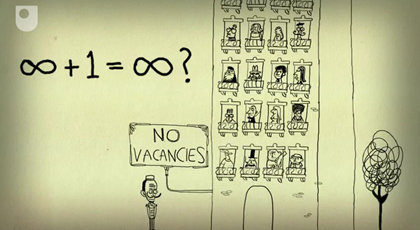
\includegraphics[width=0.5\textwidth]{BeskonacnoPlus1.jpg}
      \end{figure}
\end{itemize}
\end{frame}

\begin{frame}[fragile]\frametitle{Beskonačan broj gostiju}
\begin{itemize}
    \item Pred hotelom je sada beskonačno veliki autobus sa prebrojivo beskonačno mnogo gostiju
    \item Problem postaje nešto komplikovaniji kada treba napraviti mesta za beskonačno novih gostiju
    \item Sada će svaki gost iz sobe $n$ preći u sobu $2n$ i tako ćemo osloboditi sve sobe sa neparnim brojem
    \item Pošto neparnih brojeva ima beskonačno mnogo, ovim procesom oslobodili smo beskonačno mnogo soba
    \begin{figure}[h!]
      \centering  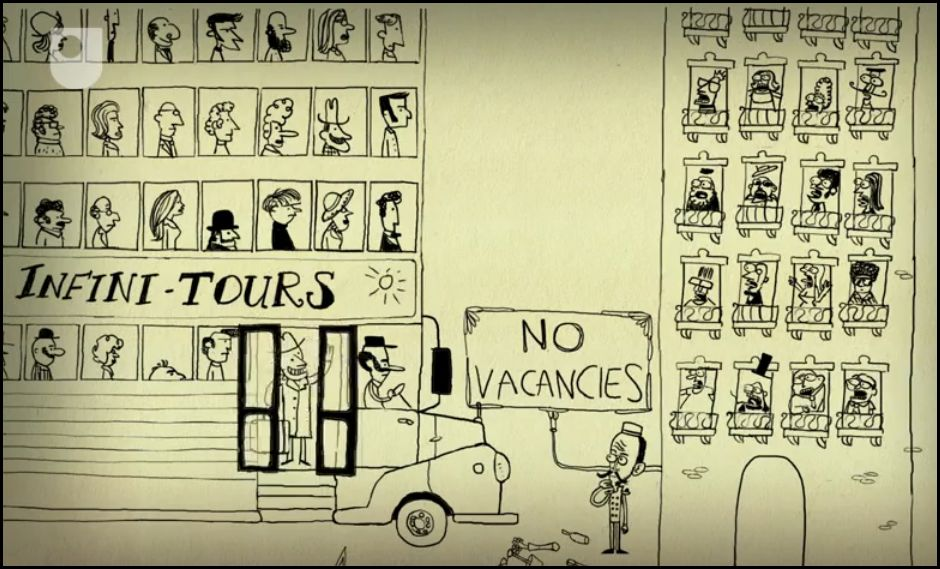
\includegraphics[width=0.4\textwidth]{BeskonacnoPlusBeskonacno.jpg}
      \end{figure}
\end{itemize}
\end{frame}

\begin{frame}[fragile]\frametitle{Beskonačan broj autobusa sa beskonačno gostiju}
\begin{itemize}
    \item Pred hotelom je sada beskonačna kolona autobus sa \textbf{prebrojivo} beskonačno mnogo putnika
    \item Da bismo smestili sve nove goste moramo da uradimo sldece korake:
    \begin{itemize}
        \item Prvo postojeće goste šaljemo u sobu sa prvim prostim brojem 2 stepenovanim brojem njihove trenutne sobe.
        \item Sada gostima iz prvog autobusa dodeljujemo sledeci prost broj 3 stepenovan brojem nihovog sedista.
        \item Putnicima iz sledeceg autobusa se dodeljuju eksponenti sledećeg prostog broja
    \end{itemize}
\end{itemize}
\end{frame}

\begin{frame}[fragile]\frametitle{Euklidov dokaz: beskonačno prostih brojeva}
\begin{itemize}
    \item Euklid je izneo dokaz da prostih brojeva ima beskonačno mnogo u svom delu „Elementi”
    \item Dat bilo koji konačni skup prostih brojeva $p_{1}, p_{2}, ..., p_{n}$
    \item $P = p_{1}p_{2}...p_{n}$
    \item Neka je $q = P + 1$. Tada $q$ ili jeste ili nije prost broj
    \begin{itemize}
        \item Ako je $q$ prost, onda postoji bar jedan broj ($q$) koji je prost, a nije u prvobitnom skupu.
        \item Ako $q$ nije prost, onda neki prost broj $p$ deli $q$. Kad bi ovaj broj $p$ bio u skupu, tada bi on delio $P$ ali bi $p$ delilo i $q$. Ako $p$ deli $P$ i $q$, onda bi $p$ morao da deli razliku ova dva broja. Posto ni jedan prost broj ne deli 1 $p$ ne može pripadati skupu.
    \end{itemize}
\end{itemize}
\end{frame}

\section{Princip neprebrojivosti}
\begin{frame}[fragile]\frametitle{Neprebrojivost}
\begin{itemize}
 \item Šta ako dolazi tura gostiju koja ne može biti numerisana prirodnim brojevima?
    \item Skup za koji je nemoguće naći bijektivnu funkciju koja preslikava skup prirodnih brojeva u dati skup naziva se \textbf{neprebrojiv} skup
    \item Jedan od takvih skupova je skup realnih brojeva
\end{itemize}
\begin{itemize}
    \item Hilbertov hotel ima prebrojivo mnogo beskonačnih soba
    \item Kada bi pokušali da smestimo neprebrojivo mnogo beskonačno gostiju u hotel ne bismo uspeli, jer neprebrojiv skup ima više elemenata nego prebrojiv skup
\end{itemize}
\end{frame}
\section{Zaključak}
\begin{frame}[fragile]\frametitle{Zaključak}
\begin{itemize}
 \item Paradoks Hilbertovog hotela nam na dobar način objašnjava značaj koncepta beskonačnosti
    \item Glavni motiv analiziranja različitih vrsta beskonačnosti i paradoksa Hilbertovog hotela je razumevanje
    skupova brojeva koje svakodnevno koristimo kao što su skup prirodnih, celih i realnih brojeva

\end{itemize}
\end{frame}

\end {document}
